\documentclass{standalone}
\usepackage{tikz}
\usetikzlibrary{calc} % for tikz calculations
\usetikzlibrary{arrows,decorations.markings} % make arrow head bigger

% set up externalization
\usetikzlibrary{external}
\tikzset{external/system call={latex \tikzexternalcheckshellescape -halt-on-error
-interaction=batchmode -jobname "\image" "\texsource" && 
dvips -o "\image".ps "\image".dvi &&
ps2eps "\image.ps"}}
\tikzexternalize[shell escape=-enable-write18] % MikTeX uses a -enable-write18 instead of --shell-escape.
% compile with: latex -enable-write18

\begin{document}

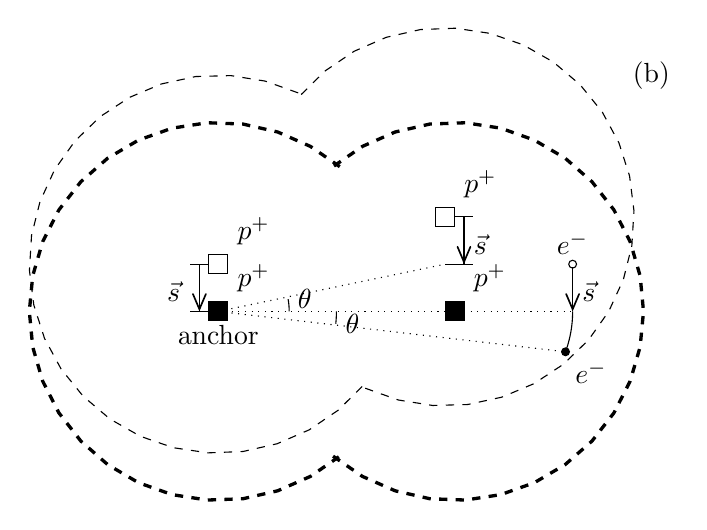
\begin{tikzpicture}
% define arrow head
[
    decoration={
      markings,
      mark=at position 1 with {\arrow[scale=1.5,black]{angle 45}};
    }
]
% scale
\pgfmathsetmacro{\a}{3}
\coordinate (H1) at (0,0);
\coordinate (H) at (\a,0);

% ions
\pgfmathsetmacro{\R}{0.04*\a} % ion radius
\draw[fill] ($(H1)-(\R,\R)$) rectangle ($(H1)+(\R,\R)$) node [above right] {$p^+$};
\draw[fill] ($(H)-(\R,\R)$) rectangle ($(H)+(\R,\R)$) node [above right] {$p^+$};
\draw [domain=50:310,dashed,very thick] plot ({0.8*\a*cos(\x)}, {0.8*\a*sin(\x)});
\draw [domain=-130:130,dashed,very thick] plot ({0.8*\a*cos(\x)+\a}, {0.8*\a*sin(\x)});
\node at ($(H1)-(0,0.1*\a)$) {anchor};

\pgfmathsetmacro{\s}{0.2*\a}
\draw[postaction={decorate}] ($(H1)+(-2*\R,\s)$) -- ($(H1)+(-2*\R,0)$);
\draw  ($(H1)+(-\R,\s)$) -- ($(H1)+(-3*\R,\s)$);
\draw  ($(H1)+(-\R,0)$) -- ($(H1)+(-3*\R,0)$) node [above left] {$\vec{s}$};
\coordinate (H1) at (0,\s);
\coordinate (H) at ($(\a-0.2*\s,2*\s)$);
% ions
\draw ($(H1)-(\R,\R)$) rectangle ($(H1)+(\R,\R)$) node [above right] {$p^+$};
\draw ($(H)-(\R,\R)$) rectangle ($(H)+(\R,\R)$) node [above right] {$p^+$};
\draw [domain=65:320,dashed] plot ({0.8*\a*cos(\x)}, {0.8*\a*sin(\x)+\s});
\draw [domain=-115:140,dashed] plot ({0.8*\a*cos(\x)+\a-0.2*\s}, {0.8*\a*sin(\x)+2*\s});

% electrons
\coordinate (e) at (1.5*\a,\s);
\node[draw,circle,inner sep=1pt] at (e) {};
\node at (e) [above] {$e^-$};
\draw[postaction={decorate}] ($(e)-(0,0.07*\s)$) -> ($(e)-(0,\s)$) node [above right] {$\vec{s}$};
\pgfmathsetmacro{\t}{20} % angle of electron
\coordinate (e1) at ({0.5*\a*cos(-\t)+\a}, {0.5*\a*sin(-\t)});
\draw [domain=0:-\t] plot ({0.5*\a*cos(\x)+\a}, {0.5*\a*sin(\x)});
\node[draw,circle,inner sep=1pt,fill] at (e1) {};
\node at (e1) [below right] {$e^-$};

% angle
\draw[postaction={decorate}] ($(H)+(2*\R,0)$) -> ($(H)-(0,\s)+(2*\R,0)$) node [above right] {$\vec{s}$};
\draw ($(H)+(\R,0)$) -- ($(H)+(3*\R,0)$);
\draw ($(H)-(0,\s)$) -- ($(H)+(3*\R,0)-(0,\s)$);
\draw[dotted] (0,0) -- ($(H)-(0,\s)$); 
\draw[dotted] (0,0) -- ($(e)-(0,\s)$); 
\draw[dotted] (0,0) -- ($(e1)$);
\draw[domain=0:10] plot ({0.3*\a*cos(\x)}, {0.3*\a*sin(\x)}) node [right] {$\theta$};
\draw[domain=0:-6] plot ({0.5*\a*cos(\x)}, {0.5*\a*sin(\x)}) node [right] {$\theta$};

% subplot marking
\node at (5.5,3) {(b)};
\end{tikzpicture}

\end{document}